\section{Sisteme de recomandare}

\subsection{Noțiuni generale}

Sistemele de recomandare au scopul de oferi sugestii de articole utilizatorilor unei platforme pe baza unor strategii. Un sistem de recomandare poate folosi una sau mai multe strategii de recomandare. 

În cazul în care se folosesc cel puțin două strategii, sistemul de recomandare devine un sistem de recomandare hibrid. Prin folosirea mai multor strategii se urmărește ca fiecare strategie să vină în completarea celorlalte cu avantajele sale.

De cele mai multe ori, în implementarea unui sistem de recomandare, se folosește tehnica de filtrare coloborativă împreună cu o altă strategie de recomandare \hyperlink{ErionCanoMaurizioMorisio}{[4]}.

\subsection{Strategii de recomandare}

\subsubsection*{Filtrarea coloborativă}

Filtrarea coloborativă se bazează pe faptul că utilizatorii care au în prezent preferințe similare vor avea și în viitor preferințe destul de similare. Această abordare folosește ratingurile pe care le dau utilizatorii sau oricare altă formă de a da un feedback, îmi place/nu îmi place, pentru a identifica preferințele comune dintre grupurile de utilizatori. Odată identificate preferințele se generează recomandări pe baza similarităților dintre utilizatori. 

Dezavantajul acestei strategii apare în momentul în care în sistem intră un nou utilizator. Datorită faptului că utilizatorul este nou, sistemul nu are un istoric al preferințelor lui, iar în consecință nu îl poate asigna unui grup de utilizatori pe baza preferințelor \hyperlink{ErionCanoMaurizioMorisio}{[4]}.

\begin{figure}[!h]
	\centering
	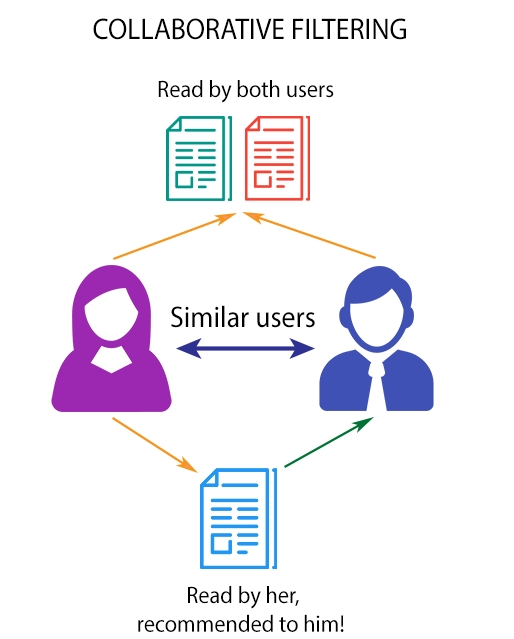
\includegraphics[max width=10cm,max height=10cm,keepaspectratio]{img_2_1}
	\caption[Filtrarea coloborativă]{Filtrarea coloborativă. Imagine preluată din \hyperlink{datameetsmedia}{[5]}.}
\end{figure} 

\subsubsection*{Filtrarea bazată pe conținut}

Filtrarea bazată pe conținut pleacă de la premisa că utiliztorii cărora le-au plăcut articole definite de anumite atribute în trecut, vor aprecia aceleași tip de articole și în viitor. Această abordare folosește atributele articolelor pentru a le compara cu profilul utilizatorilor și a oferi recomandări. Calitatea recomandărilor create folosind această strategie este influențată de setul de atribute ales pentru articole.

Similar cu filtrarea coloborativă și filtrarea bazată pe conținut prezintă dezavantaje în momentul în care în sistem intră un nou utilizator fără istoric \hyperlink{ErionCanoMaurizioMorisio}{[4]}.

\begin{figure}[!h]
	\centering
	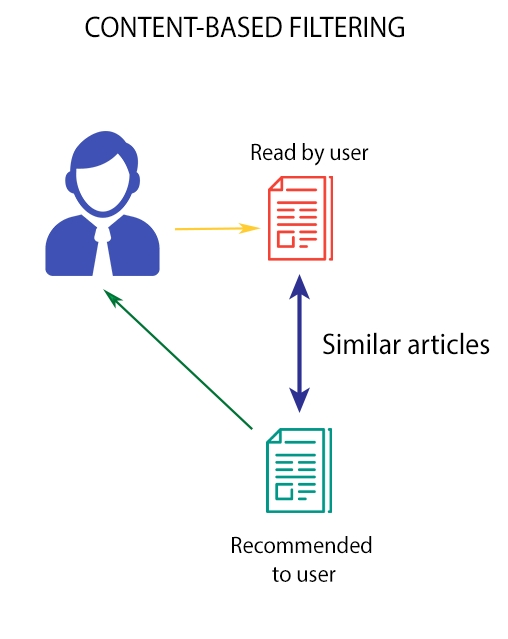
\includegraphics[max width=10cm,max height=10cm,keepaspectratio]{img_2_2}
	\caption[Filtrarea bazată pe conținut]{Filtrarea bazată pe conținut. Imagine preluată din \hyperlink{datameetsmedia}{[5]}.}
\end{figure} 

\subsubsection*{Filtrarea demografică}

Filtrarea demografică folosește atribute precum vârsta, genul, educația, etc. pentru a identifica categoriile de utilizatori. Nu prezintă dezavantaje atunci când apar noi utilizatori în sistem și nu se folosește de ratinguri, sau alt sistem de feedback, pentru a face recomandări.

Dezavantajul este reprezentat de faptul că procesul de colectare al datelor demografice poate fi îngreunat de legislație fapt ce reprezintă o limitare a acestei metode \hyperlink{ErionCanoMaurizioMorisio}{[4]}.

\subsubsection*{Filtrarea bazată pe cunoștințe}

Filtrarea bazată pe cunoștințe folosește cunoștințele despre utilizatori și articole pentru a spune ce articole îndeplinesc cerințele utilizatorilor și genereaza recomandări în consecință. Filtrare bazată pe cunoștințe are la bază constrângeri și este capabilă să recomande chiar și articole complexe care nu sunt cumpărate atât de des, precum mașini sau case \hyperlink{ErionCanoMaurizioMorisio}{[4]}.

\subsection{Funcții de loss}

\subsubsection*{BPR: Bayesian Personalised Ranking}

Este o metodă ce se bazează pe feedback implicit (click-uri, ratinguri, achiziții). Exită multe metode ce se bazează pe acest feedback implicit, precum matrix factorization (MF), k-nearest-neighbor (kNN), însă acestea nu sunt optimizate pentru ranguri. Metoda de învățare este bazată pe gradientul descendent. Metoda este recomandată atunci când se dorește optimizarea acurateții.

Definim în continuare $U$ ca fiind mulțimea de utilizatori și $I$ ca fiind mulțimea de articole. Feedback-ul implicit este reprezentat de mulțimea $S \subseteq U \times I$. De asemenea, definim $I_u^+ := {i \in I:(u, i) \in S}$ și $U_i^+ := {u \in U:(u, i) \in S}$.

\begin{figure}[!h]
	\centering
	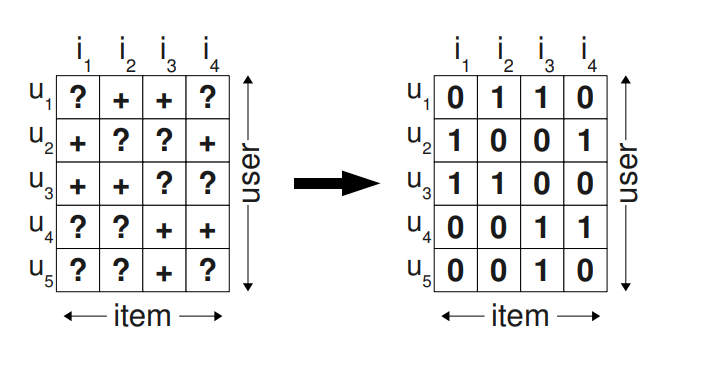
\includegraphics[max width=10cm,max height=10cm,keepaspectratio]{img_2_8}
	\caption[Matricea de interacțiuni]{Matricea de interacțiuni, mulțimea $S$. Imagine preluată din \hyperlink{SteffenRendleChristophFreudenthalerZenoGantnerLarsSchmidtThieme}{[9]}.}
\end{figure} 

O abordarea uzuală pentru recomandarea de articole este să fie prezis scorul $\hat{x}_{ui}$ care să reflecte preferința utilizatorului $u$ pentru articolul $i$. Apoi fiecare articol primește un rang după sortarea scorurilor.

Setul de antrenare este definit de mulțimea $D_S := \{(u,i,j)|i \in I_u^+ \wedge j \in I \setminus I_u^+\}$ unde $(u,i,j)$ înseamnă că utilizatorul $u$ preferă articolul $i$ în detrimentul articolului $j$.

\begin{figure}[!h]
	\centering
	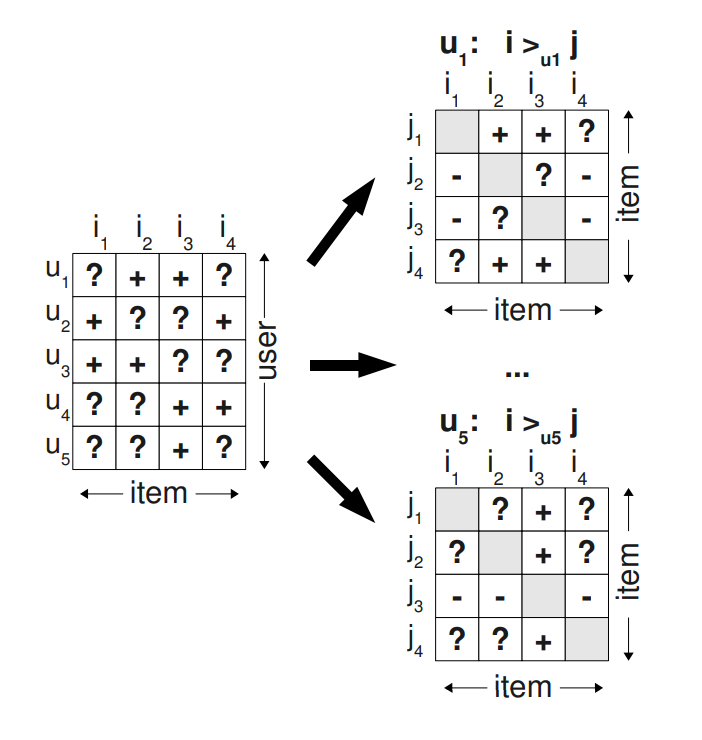
\includegraphics[max width=10cm,max height=10cm,keepaspectratio]{img_2_9}
	\caption[Setul de antrenare]{Setul de antrenare. $+$ reprezintă articolele $i$ pe care utilizatorul le preferă în locul articolelor $j$, $-$ utilizatorul preferă articolele $j$ în loc de $i$, iar $?$ reprezintă lipsa informației despre acea interacțiune. Imagine preluată din \hyperlink{SteffenRendleChristophFreudenthalerZenoGantnerLarsSchmidtThieme}{[9]}.}
\end{figure} 

Criteriul de optimizare pentru pentru rangurile personalizate este definit după cum urmează:
\begin{align}
	BPR-OPT := \sum_{(u,i,j) \in D_S} \ln{\sigma(\hat{x}_{uij})} - \lambda_\Theta||\Theta||^2
\end{align}

unde $\sigma$ este funcția sigmoid, $\sigma(x) := \frac{1}{1+e^{-x}}$, $\Theta$ reprezintă vectorul parametru al modelului care definește interacțiunea dintre utilizatorul $u$, articolul $i$ și articolul $j$, iar $\lambda_\Theta$ reprezintă parametrii de regularizare.

\vspace{5mm}
Cu aceste definiți putem defini și procedura de învățare a $BPR$ după cum urmează.

\begin{figure}[!h]
	\centering
	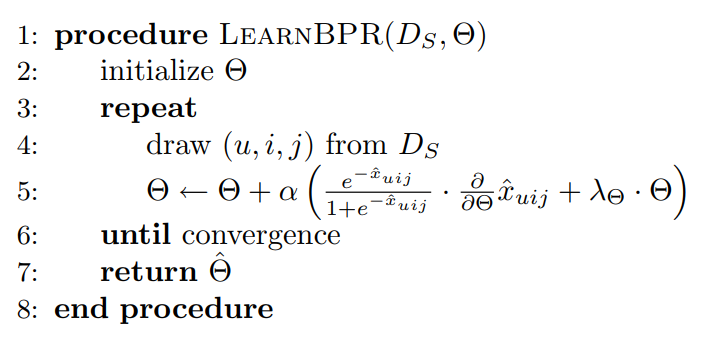
\includegraphics[max width=10cm,max height=10cm,keepaspectratio]{img_2_10}
	\caption[Procedura de învățarea BPR]{Optimizarea modelului bazată metoda gradientului descendent cu parametrul de învățare $\alpha$ și regularizarea $\lambda_\Theta$. Imagine preluată din \hyperlink{SteffenRendleChristophFreudenthalerZenoGantnerLarsSchmidtThieme}{[9]}.}
\end{figure}

\vspace{5mm}
\subsubsection*{WARP: Weighted Approximate-Rank}

Această metodă își are originile în procesarea imaginilor și anume pentru un set de reprezentări ale unor imagini $x \in R^d$ și pentru un set de reprezentări ale unor adnotări $i \in \Upsilon = \{1, ..., Y\}$ - inidici intr-un dicționar cu posibile adnotări, metoda învață să mapeze imagini din spațiul reprezentărilor într-un spațiu comun $R^D$

\begin{align}
	\Phi_{I}(x):R^d \rightarrow R^D
\end{align}

în același timp învățând și mapări pentru adnotări în același spațiu

\begin{align}
	\Phi_{W}(i):{1,...,Y} \rightarrow R^D
\end{align}

Scopul principal fiind acela de a oferi ranguri posibilelor adnotări pentru o imagine dată astfel încât cel mai mare rang să descrie cel mai bine conținutul semnatic al imaginii. 

Modelul folosit este următorul:
\begin{align}
	f_{i}(x) = \Phi_{W}(i)^T \Phi_{I}(x)
\end{align}

Metoda învață să producă ranguri optimizate pentru primele adnotări din listă, ceea ce înseamnă că optimizează precizia@k.

În ceea ce privește funcția de eroare definim: $f(x) \in R^Y$ ce produce un scor pentru fiecare etichetă și unde $f_i(x)$ este valoarea etichetei $i$. Definim funcția de eroare pentru ranguri ca fiind:
\begin{align}
	err(f(x),y) = L(rank_y(f(x)))
\end{align}
unde $rank_y(f(x))$ este rangul etichetei corecte data de $f(x)$:
\begin{align}
	rank_y(f(x)) = \sum_{i \neq y}I(f_i(x) \geq f_y(x))
\end{align}
unde I este funcția indicator, iar $L(\cdot)$ transformă rangul în penalizare
\begin{align}
	L(k) = \sum_{j=1}^k\alpha_j, \quad cu \quad \alpha_1 \geq \alpha_2 \geq ... \geq 0.
\end{align}

$L(\cdot)$ poate lua diferite forme în funcție de ce se dorește a se optimiza: $\alpha_j=\frac{1}{Y-1}$ optimizează rangul mediu, $\alpha_j=1$ și $\alpha_{j>1}=0$ optimizează proporția de ranguri corecte aflate în top, iar valorile mari ale lui $\alpha$ optimizează primele $k$ în lista de ranguri\hyperlink{JasonWestonSamyBengioNicolasUsunier}{[8]}.

\vspace{5mm}

Cu definițiile prezentate mai sus putem descrie algoritmul acestei metode după cum urmează.

\begin{figure}[!h]
	\centering
	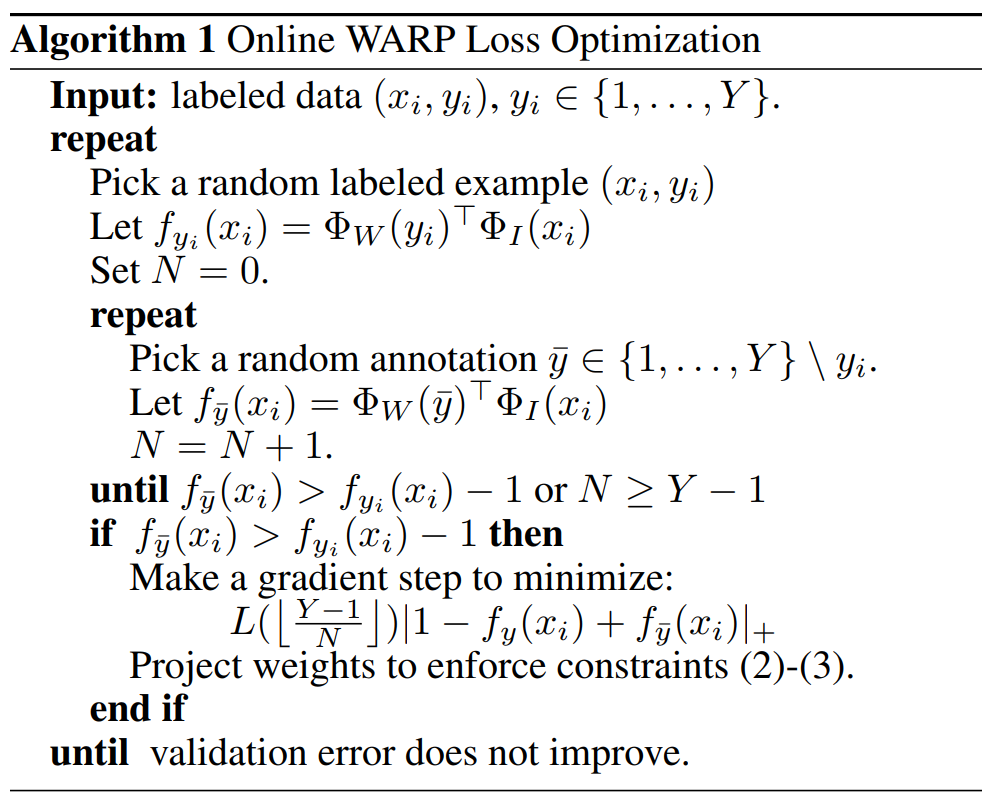
\includegraphics[max width=10cm,max height=10cm,keepaspectratio]{img_2_7}
	\caption[Online WARP Loss Optimization]{Online WARP Loss Optimization. Imagine preluată din \hyperlink{JasonWestonSamyBengioNicolasUsunier}{[8]}.}
\end{figure} 

\section{Rețele neurale convoluționale}

\subsection{Noțiuni generale}

Rețelele neurale convoluționale sunt foarte similare cu rețelele neurale fiind formate din neuroni ce învață ponderi ($w$) și baiasuri ($b$). Scopul rețelei convoluționale este de a primi o imagine la input și de a scoate la output un scor pentru fiecare clasă ce corespunde imaginii. 

Spre exemplu, la input se dă o imagine cu un autovehicul, iar rețeaua convoluțională poate spune că în imagine este o mașină în proporție de 80\%, un camion în proporție de 10\%, un avion în proporție de 6\%, o barcă în proporție de 3\% sau un cal în proporție de 1\%.

\begin{figure}[!h]
	\centering
	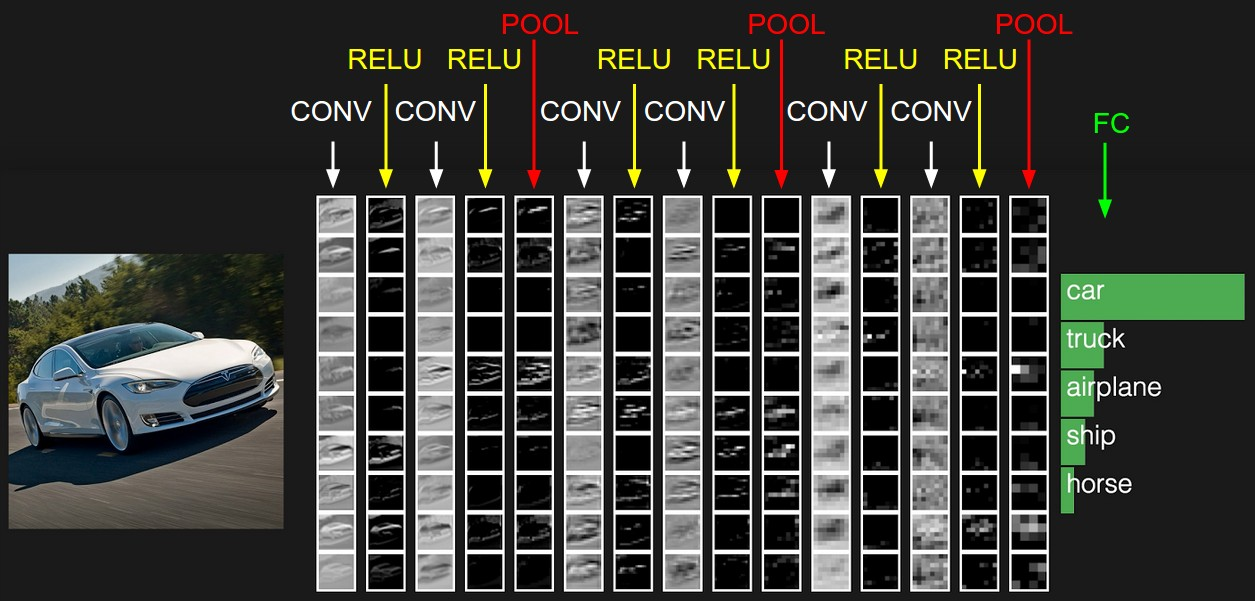
\includegraphics[max width=10cm,max height=10cm,keepaspectratio]{img_2_3}
	\caption[Exemplu rețea convoluțională]{Exemplu de rețea convoluțională care primește la input o imagine și produce la output o listă de clase ce pot descrie imaginea de input. Imagine preluată din \hyperlink{datameetsmedia}{[7]}.}
\end{figure} 

Rețelele convoluționale sunt compuse dintr-o secvență de layere ce poate fi împărțită în trei tipuri principale de layere \hyperlink{cs231n}{[7]}:

\begin{enumerate}
  \item Convolutional Layer este layerul de bază într-o rețea convoluțională. Parametrii acestui layer sunt reprezentați de filtre învățabile, unde fiecare filtru reprezintă o mică bucată din imaginea de input. De exemplu, un filtru pentru pentru acest layer poate avea dimensiunea de $5\times5\times3$, dimensiune ce reprezintă faptul că se iau 5 pixeli pe lațime și înălțime cu o adâncime de 3, unde adâncimea reprezintă canalele RGB. În continuare se glisează fiecare filtru peste input și se compune produsul dintre filtre și input la fiecare poziție. În urma acestei operații se produce un vector de activare 2-dimensional care reprezintă răspunsul filtrului la fiecare poziție. Altfel spun, rețeaua va învăța filtre care se activează atunci când sunt prezente anumite tipuri de caracteristici, precum culoarea sau orientarea.

\begin{figure}[!h]
	\centering
	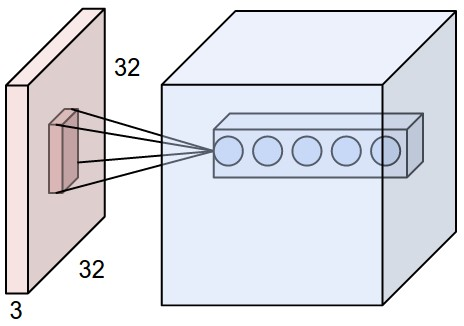
\includegraphics[max width=10cm,max height=10cm,keepaspectratio]{img_2_4}
	\caption[Exemplu de filtru aplicat peste input]{Exemplu de filtru aplicat peste input într-un layer convoluțional. Imagine preluată din \hyperlink{datameetsmedia}{[7]}.}
\end{figure}   
  
  \item Pooling Layer reprezintă o practică des folosită între mai multe layere convoluționale succesive. Această operație reduce numărul de parametrii (dimensiunea), computațiile din rețea și controlează overfittingul. Se execută indepedent pe fiecare nivel al adâncimii unui input și pastrează valoarea maximă a acelei zone. Rezultatul este o zonă de caracteristicii mai mică dar care păstrează cea mai relevantă statistică.

\begin{figure}[!tbp]
  \begin{subfigure}[b]{0.4\textwidth}
    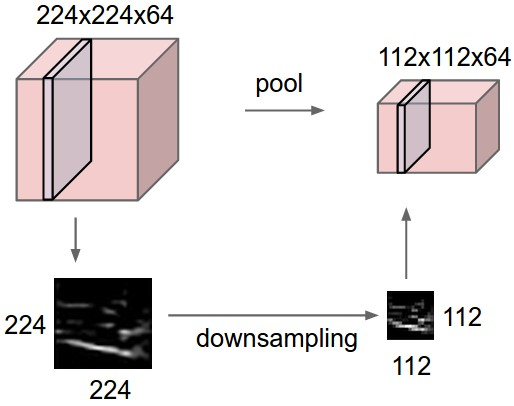
\includegraphics[width=\textwidth]{img_2_5}
    \caption{Reducerea dimensiunii.}
    \label{fig:f1}
  \end{subfigure}
  \hfill
  \begin{subfigure}[b]{0.4\textwidth}
    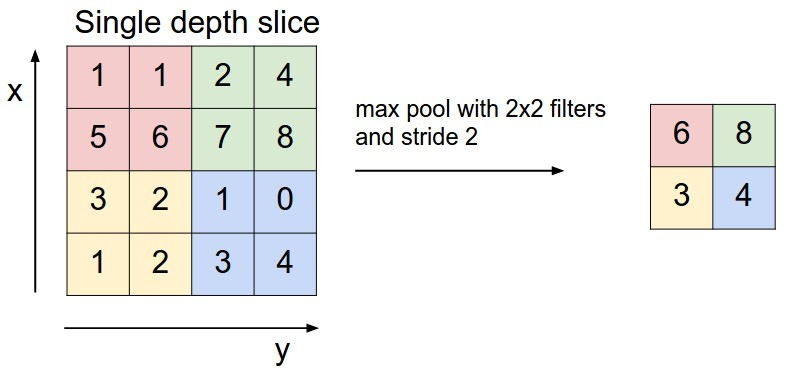
\includegraphics[width=\textwidth]{img_2_6}
    \caption{Filtrul de $2\times2$ aplicat ce păstrează valoarea maximă.}
    \label{fig:f2}
  \end{subfigure}
  \caption[Exemplu de pooling]{Exemplu de pooling. Imagine preluată din \hyperlink{datameetsmedia}{[7]}.}
\end{figure}
  
  \item Fully-Connected Layer este stratul în care caracteristicile sunt vectorizate pentru a putea fi folosite.
\end{enumerate}

\subsection{VGG}

VGG este o arhitectură de rețea cu filtre convoluționale foarte mici, de dimensiune $3\times3$ și care poate avea o adâncime a straturilor de ponderi de 16 - 19.

În ceea ce privește arhitectura, inputul în rețeaua convoluțională este de dimensiune fixă și anume $224\times224$ imagine RGB. Mai departe, imaginea este trecută printr-un set de straturi convoluționale unde sunt utilizate filtre de dimensiune mică, $3\times3$ - fiind cea mai mică dimensiune ce poate captura noțiunile de stânga/dreapta, sus/jos, centru. Într-una dintre configurații se utilizează un filtru convoluțional de dimensiune $1\times1$. Pasul în straturile convoluționale este fixat la 1 pixel.

Poolingul este compus din cinci straturi de max-pooling care urmează după unele straturi convoluționale. Max-poolingul este calculat cu ferestre de $2\times2$ pixel și cu pas de 2 pixeli.

Odată trecută imaginea prin straturile convoluționale și cele de pooling ajunge în trei straturi fully-connected. Primele două straturi au câte 4096 de canale fiecare, iar al treilea are 1000 de canale. Canalele celui de-al treilea strat sunt asociate claselor, fiecare canal reprezintă o clasă.

Ultimul strat din rețea este un strat soft-max \hyperlink{SimonyanKarenZissermanAndrew}{[10]}.

\begin{figure}[!h]
	\centering
	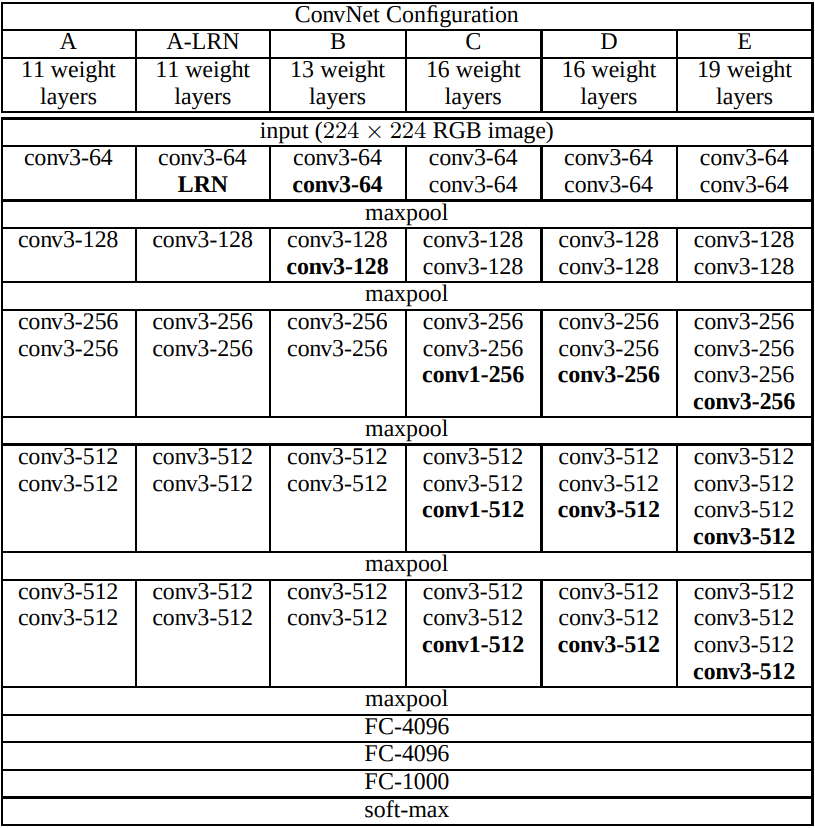
\includegraphics[max width=12cm,max height=12cm,keepaspectratio]{img_2_11}
	\caption[Configurații VGG]{Configurații ale rețelei VGG. Imagine preluată din \hyperlink{SimonyanKarenZissermanAndrew}{[10]}.}
\end{figure}   

\subsection{InceptionV3}
Prima arhitectura de Inception a apărut sub numele de GoogLeNet. O a doua versiune de Inception a fost definită prin introducerea de batch-uri normalizate. Iar mai apoi, versiunea a treia în care a fost adăugate idea de factorizare.

Factorizarea în filtre convoluționale mici presupune înlocuirea stratului cu filtru de dimensiune $5 \times 5$ cu două straturi de dimensiune $3 \times 3$ astfel reducânduse dimensiunea de la $5 \times 5 = 25$ la $3 \times 3 + 3 \times 3 = 18$.
\begin{figure}[!h]
	\centering
	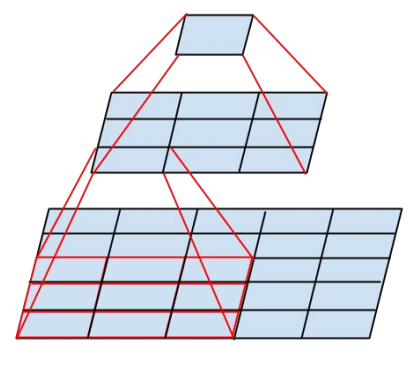
\includegraphics[max width=7cm,max height=7cm,keepaspectratio]{img_2_17}
	\caption[Factorizarea în filtre convoluționale mici]{Factorizarea în filtre convoluționale mici. Filtrul de dimensiune $5 \times 5$ înlocuit cu două de dimensiune $3 \times 3$.  Imagine preluată din \hyperlink{guideinceptionv3}{[14]}.}
\end{figure}   

Factorizarea spațială în convoluții asimetrice presupune înlocuirea stratului cu filtru de dimensiune $3 \times 3$ cu două straturi de dimensiune $3 \times 1$ și $1 \times 3$ astfel reducânduse dimensiunea de la $3 \times 3 = 9$ la $3 \times 1 + 1 \times 3 = 6$. 
\begin{figure}[!h]
	\centering
	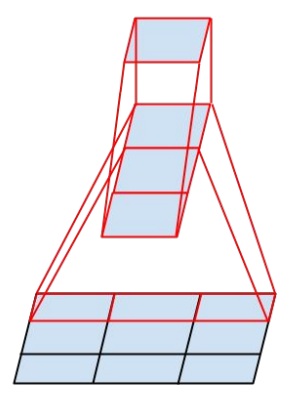
\includegraphics[max width=7cm,max height=7cm,keepaspectratio]{img_2_18}
	\caption[Factorizarea spațială în convoluții asimetrice]{Factorizarea în filtre convoluționale mici. Filtrul de dimensiune $3 \times 3$ înlocuit cu două de dimensiune $3 \times 1$ și $1 \times 3$.  Imagine preluată din \hyperlink{guideinceptionv3}{[14]}.}
\end{figure}

Clasificatori auxiliari ...

Reducerea eficientă a dimensiunii ...

\begin{figure}[!h]
	\centering
	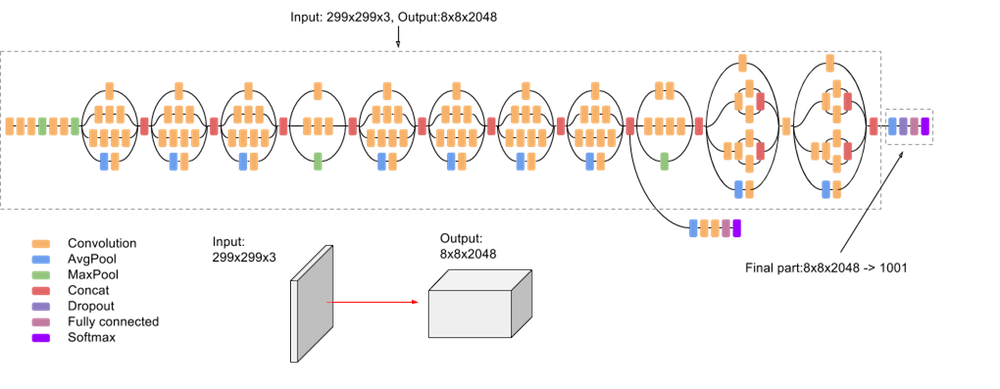
\includegraphics[max width=17cm,max height=12cm,keepaspectratio]{img_2_16}
	\caption[Arhitectura InceptionV3]{Arhitectura rețelei InceptionV3. Imagine preluată din \hyperlink{guideinceptionv3}{[14]}.}
\end{figure}   


\subsection{ResNet}
Fie $H(x)$ maparea de bază unde $x$ reprezintă inputul. Funcția reziduală poate fi aproximată cu $F(x) := H(x) - x$, maparea de bază fiind $F(x) + x$.

\begin{figure}[!h]
	\centering
	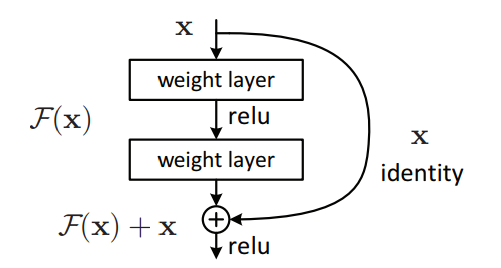
\includegraphics[max width=10cm,max height=10cm,keepaspectratio]{img_2_12}
	\caption[Învățarea reziduală]{Învățarea reziduală. Imagine preluată din \hyperlink{KaimingHeXiangyuZhangShaoqingRenJianSun}{[11]}.}
\end{figure}  

Învățarea reziduală se aplică la câtva grupuri de straturi. Putem defini un bloc de straturi ca fiind 
\begin{align}
	y = F(x,\{W_i\}) + x
\end{align}
unde $x$ și $y$ reprezintă inputul și outputul straturilor considerate. Funcția $F(x, \{W_i\})$ reprezintă maparea reziduală ce trebuie învățată.

Dimensiunea lui $x$ și $F$ din ecuația de mai sus trebuie să fie egale. Redefinim ecuația după cum urmează
\begin{align}
	y = F(x,\{W_i\}) + W_sx
\end{align}
unde $W_s$ este o proiecție liniară a scurtăturilor conexiunilor pentru ca dimensiunile să se potrivească.

ResNet pleacă de la o rețea simplă. Rețeaua simplă fiind inspirată de rețeaua VGG. Straturile convoluționale au în general filtre de dimensiune $3\times3$ și se bazează de două reguli de design: - pentru outputuri cu același număr de caracteristici, straturile vor avea același număr de filtre; - dacă numărul de caracteristicii este injumătățit, numărul de filtre este dublat astfel încât să fie păstrată complexitatea de timp pe strat.

Poolingul se realizează dupa straturile convoluționale cu un pas de 2 pixeli. Rețeaua se termină cu un strat de pooling mediu și un strat fully-connected softmax cu 1000 de canale.

Bazată pe rețeaua descrisă mai sus, rețeaua reziduală presupune inserția unor scurtături. Scurtăturile identice (vezi formula 2.8) pot fi direct utilizate când inputul și outputul au aceași dimensiune. Când dimensiunea crește considerăm două opțiuni: - scurtătura calculează în continuare maparea identității. Această opțiune nu introduce parametrii noi; - proiecția scurtăturii din formula 2.9 este utilizată pentru a potrivi dimensiunile. În ambele situații când se folosesc scurtăturile pentru pentru a sări peste două straturi sunt calculate cu un pas de 2.

\begin{figure}[!h]
	\centering
	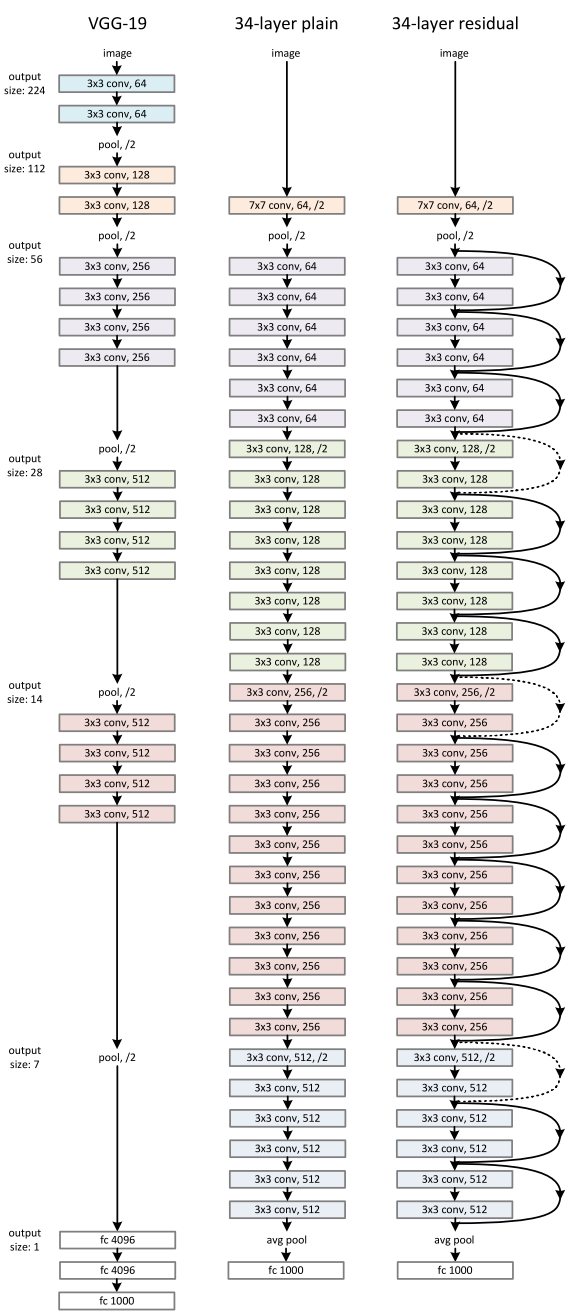
\includegraphics[max width=10cm,max height=20cm,keepaspectratio]{img_2_13}
	\caption[Rețeaua ResNet]{Prima rețea (stânga) este o rețea VGG19. A doua rețea (centru) este o rețea simplă cu 34 de straturi. A treia rețea (dreapta) este o rețea reziduală cu 34 de straturi. Imagine preluată din \hyperlink{KaimingHeXiangyuZhangShaoqingRenJianSun}{[11]}.}
\end{figure}  


\subsection{NASNet}
NASNet este o arhitectură de rețea bazată pe tehnica de căutare Neural Architecture Search (NAS). NAS presupune un controler cu o rețea neurală recurentă care conține mai multe rețele copii cu arhitecturi diferite. Rețelele copii sunt antrenate să conveargă pentru a obține o anumită precizie pe un set de antrenare. Rezultatele sunt utilizate pentru a actualiza controlerul ceea ce înseamnă că acest controler va genera arhitecturi mai bune în timp.

\begin{figure}[!h]
	\centering
	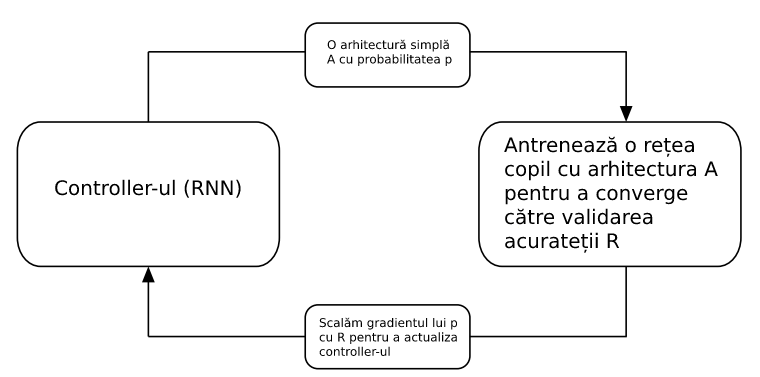
\includegraphics[max width=10cm,max height=20cm,keepaspectratio]{img_2_14}
	\caption[NAS]{Privire de ansamblu asupra unei Neural Architecture Search. Imagine preluată din \hyperlink{Zoph2018LearningTA}{[13]}.}
\end{figure}  

Plusul principal pe care îl aduce rețeaua NASnet este reprezentat de proiectarea unui nou spațiu de căutare astfel încât cea mai bună arhitectură pe setul de date CIFAR-10 poate scala către rezoluții ale imaginilor cât mai mari într-un interval definit. Astfel, acest spațiu poartă numele de \textit{NASNet search space}. În abordarea NASNet arhitecturile rețelelor convoluționale manual predeterminate, fiind compuse din celule convoluționale repetate de multe ori unde, fiecare celulă convoluțională are aceași arhitectură dar ponderi diferite.

Pentru a construi mai ușor arhitecturi scalabile pentru imagini de orice dimensiune este nevoie de două tipuri de celule convoluționale pentru a îndeplini două funcții principale: - celule convoluționale care returnează o hartă de caracteristici cu aceași dimensiune. Acest tip de celule se numesc \textit{Celulă Normal}; - celule convoluționale care returnează o hartă de caracteristici cu înălțimea și lungimea harții divizată cu un factor doi. Acest tip de celule se numesc \textit{Celulă de reducere}.

\begin{figure}[!h]
	\centering
	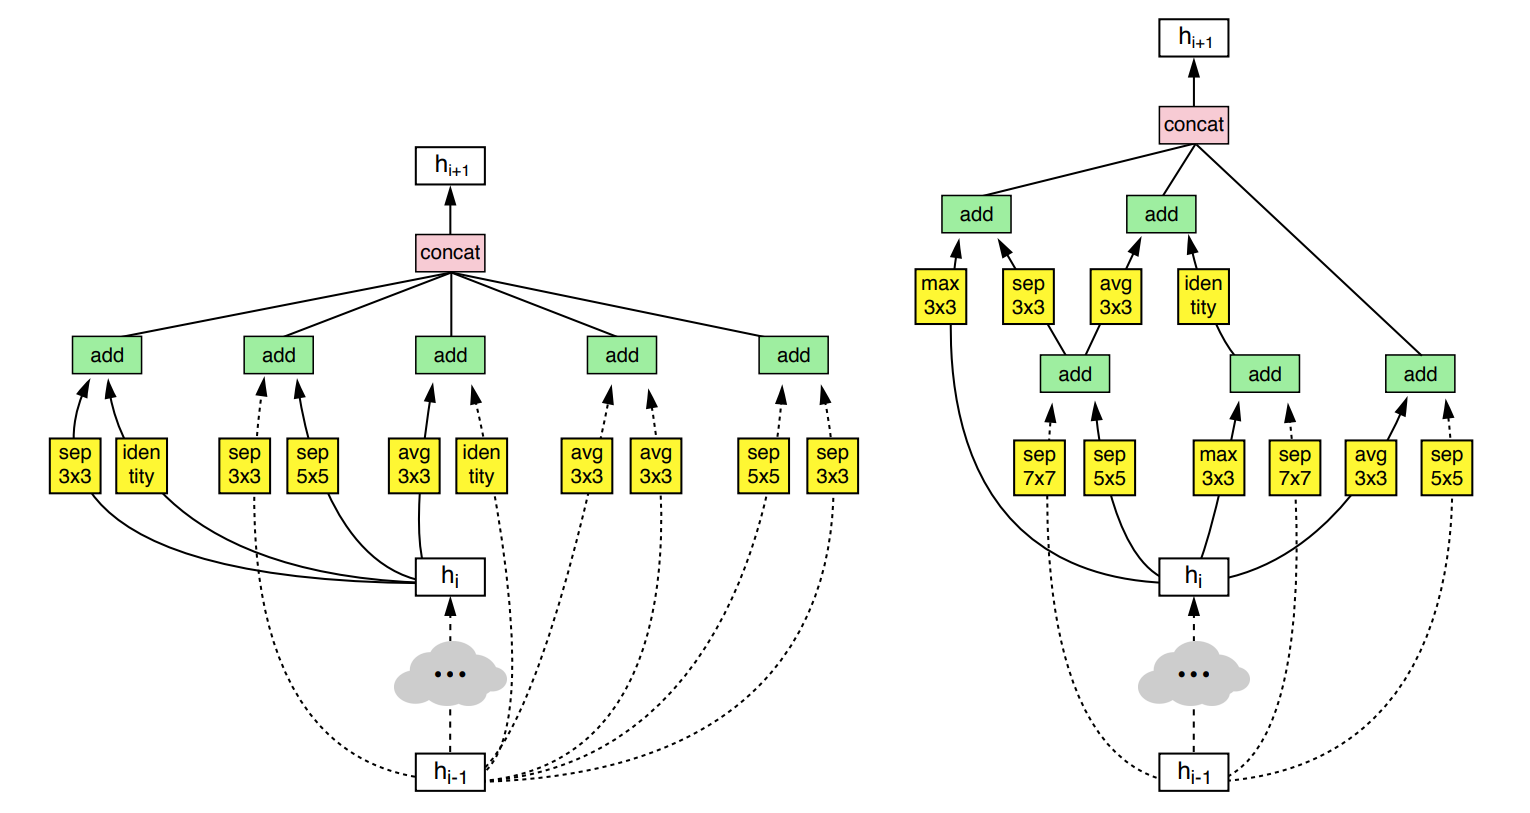
\includegraphics[max width=17cm,max height=17cm,keepaspectratio]{img_2_15}
	\caption[Celule normale și de reducere]{Celule normale (dreapta). Celule de reducere (stânga). Imagine preluată din \hyperlink{Zoph2018LearningTA}{[13]}.}
\end{figure}  

\section{Clustere}

\subsection{Noțiuni generale}

\subsection{K-nearest neighbors}
